\chapter{User Guide}

The user guide is a tutorial for non-technical users to learn how to use the tool. The tool has been extensively tested on Linux, the tool has full functionality on Linux and basic functionality on Windows.

\section{Installation}

The tool has the following required dependencies:

\begin{itemize}
	\item Python 3
	\item Tkinter
	\item NumPy
	\item Matplotlib
	\item Pillow
\end{itemize}

Tkinter is the default GUI package for Python and Matplotlib depends on NumPy so Tkinter and Matplotlib do not need to be installed explicitly. The tool has the following optional dependencies:

\begin{itemize}
	\item Pyomo
	\item An optimiser, either CPLEX or GLPK
\end{itemize}

The optional dependencies are used to optimise schedules, these are not strictly required as users can input their own schedules. GLPK is recommended because of its licence and open-source development. The repository is found at \texttt{gitlab.doc.ic.ac.uk/mtl115/aes}. Please refer to the package's websites for troubleshooting. Alternatively, contact the author for assistance.

\subsection{Linux Installation}

The tool was tested on Ubuntu 18.04.1. Python is pre-installed so the following packages can be installed as below:
\begin{verbatim}
apt install python3-pip
apt install python-glpk
apt install glpk-utils
pip3 install matplotlib
pip3 install pillow
pip3 install pyomo
\end{verbatim}

\subsection{Windows Installation}

The tool was tested on Windows 10. First, download Python from the official website, then setup the path environment variable so \texttt{python} can be executed on the command prompt. Afterwards, install the required dependencies as below: 

\begin{verbatim}
python -m pip install matplotlib
python -m pip install pillow
python -m pip install pyomo
\end{verbatim}

\section{Usage}

\subsection{Getting Started}

\begin{figure}[H]
	\centering
	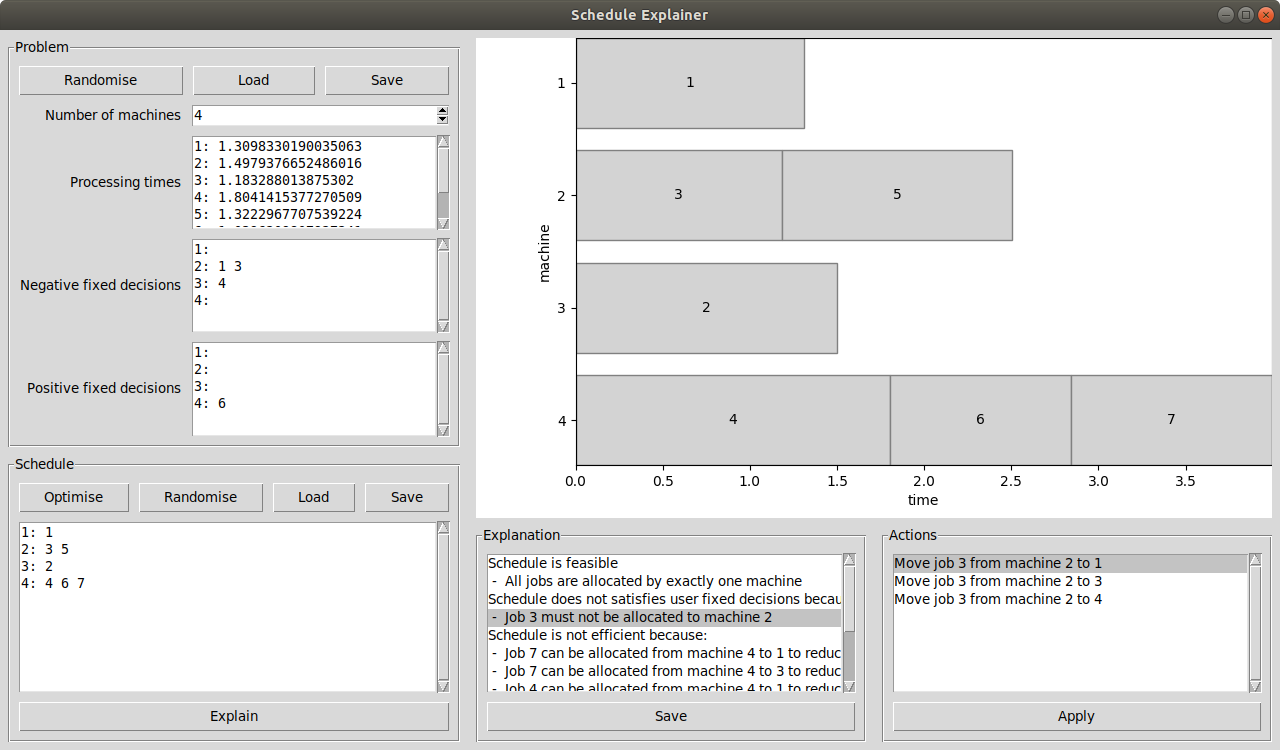
\includegraphics[width=\linewidth]{figures/tool_gui.png}
	\caption{Tool GUI}
\end{figure}

To start the tool, run \texttt{python3 main.py -g} on Linux or \texttt{python main.py -g} on Windows in the \texttt{src} directory supplied in the repository.
\linespace
The makespan problem consists of the number of machines and job processing times. The tutorial will use a hospital setting, where nurses and patients are represented as machines and jobs respectively. Consider the following example where there are two nurses, Alice and Bob. and two patients, Charlie and Dave. Charlie's and Dave's appointment takes 15 and 10 minutes respectively. To enter the example in the tool, nurses and patients are indexed. Hence, A represents Alice, B represents Bob for nurses and 1 represents Charlie and 2 represents Dave for patients. Numbers are used to index machines and letters are used to index jobs. The problem is to minimise the total completion time, which intuitively is the longest time any nurse has to work.

\begin{figure}[H]
	\centering
	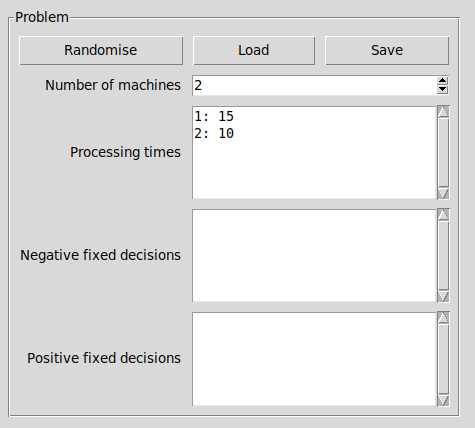
\includegraphics[scale=0.5]{figures/tool_problem.png}
	\caption{Example problem input}
\end{figure}

Each line in the processing time textbox represents one job. The first line can be interpreted as: job A has processing time of 15 units, with following lines having similar interpretations. Negative fixed decisions represent jobs that cannot be assigned to machines. Positive fixed decisions represents jobs that much be assigned to a machine. Note that for all multi-line inputs, each line ends with a new line character.

\begin{figure}[H]
	\centering
	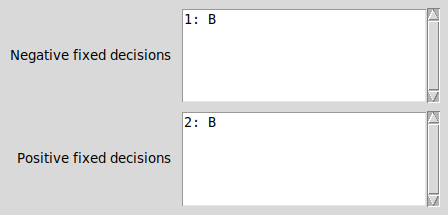
\includegraphics[scale=0.5]{figures/tool_fd.png}
	\caption{Example fixed decisions input}
\end{figure}

Each line in each fixed decisions textbox represents one decision. The first line of negative fixed decisions can be interpreted as: machine 1 cannot be allocated to job B. The first line of positive fixed decisions can be interpreted as: machine 2 cannot be allocated to job B. In context of the example, this means Alice cannot be with Dave and Bob must be with Dave.

\begin{figure}[H]
	\centering
	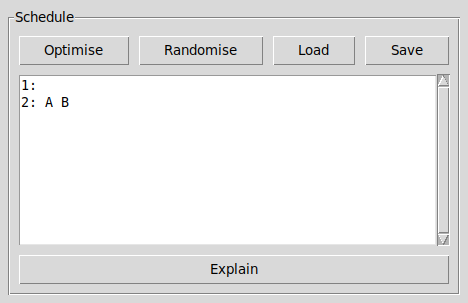
\includegraphics[scale=0.5]{figures/tool_schedule.png}
	\caption{Example schedule input}
\end{figure}

After defining the makespan problem, enter the above schedule. The schedule can be interpreted as: machine 1 has no allocated jobs; machine 2 have two allocated jobs, A and B. The \texttt{Optimise} button finds the optimal schedule using a solver, which is by default GLPK. To specify a solver, starting the tool with \texttt{python3 main.py -g -S SOLVER\_NAME} where \texttt{SOLVER\_NAME} is GLPK or CPLEX, for instance. Note that for large problems, optimisation may take a long time, so a solver time limit can be enforced by starting the tool with \texttt{python3 main.py -g -t TIME\_LIMIT} where \texttt{TIME\_LIMIT} is in seconds. The \texttt{Randomize} button generates some feasible schedule, which may violate fixed decisions. To explain the schedule, click the \texttt{Explain} button. 

\begin{figure}[H]
	\centering
	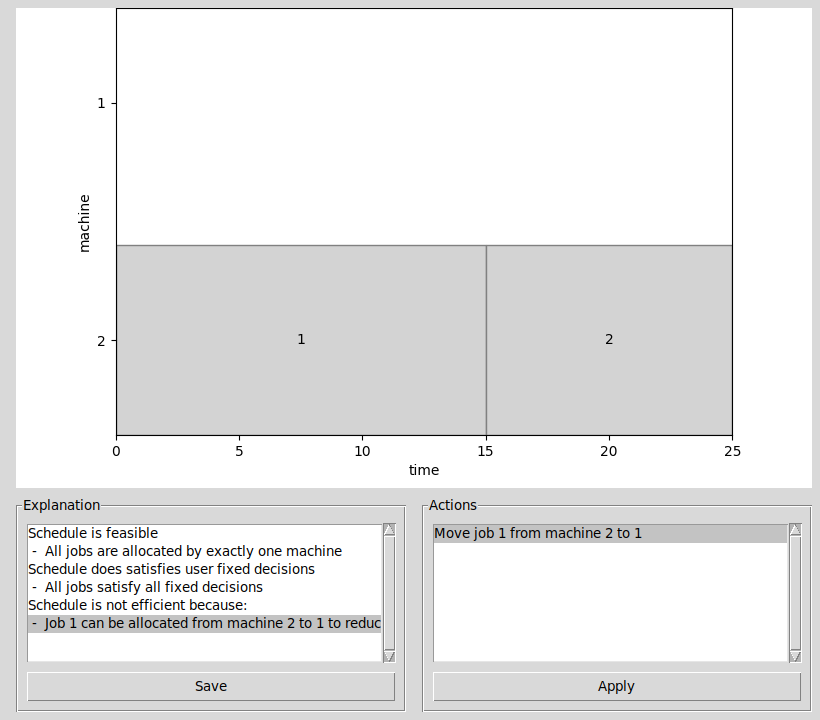
\includegraphics[width=\linewidth]{figures/tool_explain.png}
	\caption{Example explanation output}
\end{figure}

The explanation reasons on three concepts: feasibility, satisfaction of fixed decisions and efficiency. Feasibility ensures that each job is allocated once. Satisfaction of fixed decisions ensures the schedule does not violate negative and positive fixed decisions specified in the problem. Efficiency regards suggestions to improve the total completion time. To improve the schedule, select a line in the explanation listbox to address, then select a line in the actions listbox. An line of explanation may have many different approaches to address the problem or schedule. Click on the \texttt{Apply} button to improve the schedule.

\begin{figure}[H]
	\centering
	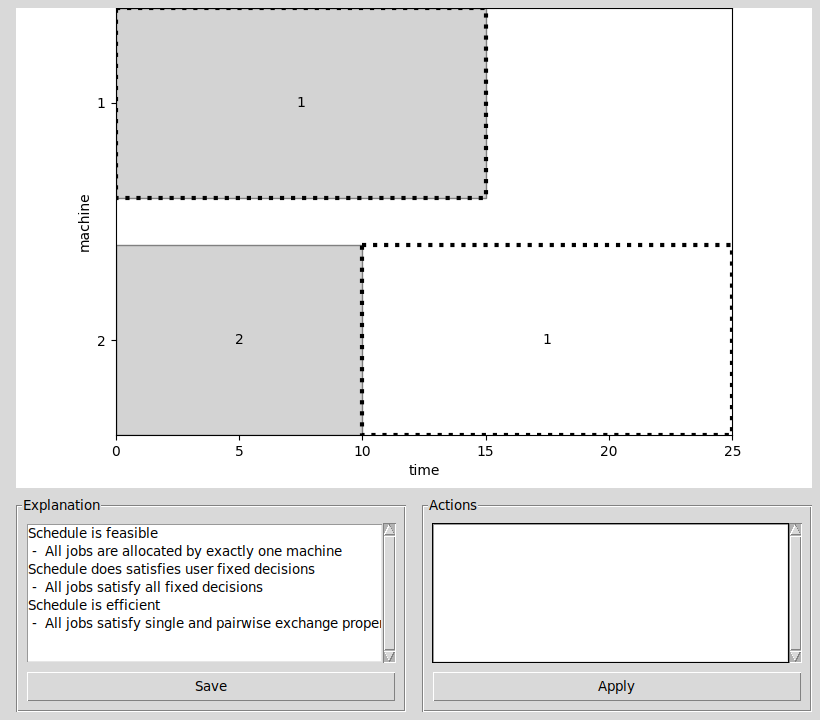
\includegraphics[width=\linewidth]{figures/tool_improve.png}
	\caption{Example explanation output}
\end{figure}

The example schedule only required one action to make the schedule efficient. However, many iterative actions may be required to reach an efficiency schedule. No further actions show that the schedule is feasible, satisfies fixed decisions and is efficient. The dot-highlighted boxes in the cascade chart illustrate newly and removed allocations compared to before the applying the action.

\subsection{Command Line Examples}

\subsubsection{Help Command}

\begin{verbatim}
> python3 main.py -h
usage: main.py [-h] [-g] [-e] [-p PROBLEM | -r [M]]
    [-O | -s SCHEDULE | -R] [-o OUTPUT] [--partial]
    [-t TIME_LIMIT] [-S SOLVER_NAME]

Explains makespan schedules using abstract argumentation
frameworks

optional arguments:
-h, --help            show this help message and exit
-g, --graphical       displays graphical user interface
-e, --explain         generate explanation
-p PROBLEM, --problem PROBLEM
-r [M], --random_problem [M]
    creates random problem with jobs and fixed decisions
    where M is the number of machines
-O, --optimise        uses SOLVER_NAME to find most efficient
schedule
-s SCHEDULE, --schedule SCHEDULE
-R, --random_schedule
-o OUTPUT, --output OUTPUT
    output filename for selected problem, schedule or
    explanation
--partial             use partial framework construction to
favour memory over CPU
-t TIME_LIMIT, --time_limit TIME_LIMIT
    maximum time for optimisation in seconds, use negative
    time_limit for infinite limit, default is unlimited
time
-S SOLVER_NAME, --solver SOLVER_NAME
    optimisation solver for schedule, default is 'glpk'
\end{verbatim}

\subsubsection{Random problem}

\begin{verbatim}
> python3 main.py -r
4;
A: 1.822
B: 2.994
C: 6.444
D: 2.578
E: 2.386
;
1: B
2: A
3: D
4: B
;
1: 
2: B
3: C
4:
\end{verbatim}

Formally, this represents $m=4$, $n=5$, $\mathbf{p}=\begin{bmatrix}
	1.822&2.994&6.444&2.578&2.386
\end{bmatrix}^T$, $D^-=\{\pair{1}{2},\pair{2}{1},\pair{3}{4},\pair{4}{2}\}$ and $D^+=\{\pair{2}{2}, \pair{3}{3}\}$.

\subsubsection{Random schedule given previous problem}

\begin{verbatim}
> python3 main.py -p example.problem -R
1: A
2: B C E
3: D
4: 
\end{verbatim}

Formally, this represents $\mathbf{x}=\begin{bmatrix}
	1&0&0&0&0\\
	0&1&1&0&1\\
	0&0&0&1&0\\
	0&0&0&0&0\\
\end{bmatrix}$

\subsubsection{Explantation given previous problem and schedule}

\begin{verbatim}
> python3 main.py -p example.problem -s example.schedule -e
Schedule is feasible
-  All jobs are allocated by exactly one machine
Schedule does not satisfies user fixed decisions because:
-  Job C must be allocated to machine 3
-  Job D must not be allocated to machine 3
Schedule is not efficient because:
-  Job C can be allocated from machine 2 to 4 to reduce by 5.38
-  Jobs C and D can be swapped with machines 2 and 3 to reduce by 3.87
-  Job C can be allocated from machine 2 to 1 to reduce by 3.56
-  Job C can be allocated from machine 2 to 3 to reduce by 2.8
-  Job E can be allocated from machine 2 to 1 to reduce by 2.39
-  Job E can be allocated from machine 2 to 3 to reduce by 2.39
-  Job E can be allocated from machine 2 to 4 to reduce by 2.39
\end{verbatim}

\section{Known Limitations}

\begin{itemize}
	\item Holding down space for a button that requires significant computation results in permanent depressed visual of the button. This is a issue with Tkinter.
\end{itemize}